\documentclass[ ]{article}
\usepackage[ ]{graphicx}
\usepackage[ ]{indentfirst}
\title{Revisão P1\\Sistemas Operacionais}
\author{Erickson Müller}
\date{03 de outubro}

\begin{document}
	\maketitle
	\section*{Conteúdos}
		\begin{enumerate}
			\item Processosl
			\item Threads
			\item Impasses
			\item Gerenciamento de memória
		%	\item Tratamento de entrada e saída
		\end{enumerate}
	\newpage
	\section{Processos}
	
		O sistema operacional tem o modo kernel/supervisor e o modo usuário, o único ator que roda em modo kernel é o SO.
		
		Árvore de processos. O sistema operácional usa a hierariquia de processos para reservar a memória, carregar as partes do processo.
		
		O primeiro processo da árvore inicia o sistema operacional
		
		Os processos podem criar algum processo filho para caso necessite abrir outro programa para executar o comando.
		
		O pipe é um canal de comunicação entre dois processos.
		
		Um processo é a instanciação de um arquivo executável.
		\subsection{Preemptividade}
			A multiprogramação permite executar múltiplos processos "ao mesmo tempo", na realidade todos os processos são executados em um ciclo de \textit{50ms} por vez. O \textit{timer} da cpu é responsável por calcular esse ciclo, o timer é uma parte de hardware que tem um clock de 1hz e vai decrescendo de 50 até 0.
			
			Em sistemas operacionais, uma troca de contexto (também conhecido como chaveamento ou mudança de contexto) é o processo computacional de armazenar e restaurar o estado (contexto) de uma CPU de forma que múltiplos processos possam compartilhar uma única instância de CPU.
			
			Cada thread tem  sua própria pilha.
			
		\subsection{Modelo em quatro partes}
		O espaço de endereçamento da memória de um processo é dividido em quatro partes:
			\begin{enumerate}
				\item Code/Text
				\item Data
				\item Heap/Lacuna
				\item Stack/Pilha
			\end{enumerate}
			
		Pilha e Heap crescem em sentidos opostos.
		\subsection{Modelo em três partes}
		O espaço de endereçamento da memória de um processo é dividido em três partes:
			\begin{enumerate}
				\item Code/Text
				\item Stack/Pilha
				\item Heap + Data
			\end{enumerate}
			
		Pilha e Heap crescem em sentidos opostos.
	\section{Threads}
		\subsection{Região Crítica}
		
		Condições para a solução de uma \textbf{exclusão mútua}:
		\begin{itemize}
			\item Nunca dois processos simultaneamente em uma
região crítica.
			\item Nenhuma afirmação/exigência sobre
velocidades ou números de CPUs.
			\item Nenhum processo executando fora de sua
região crítica pode bloquear outros processos
			\item Nenhum processo deve esperar eternamente
para entrar em sua região crítica (deadlock??)
		\end{itemize}
		
		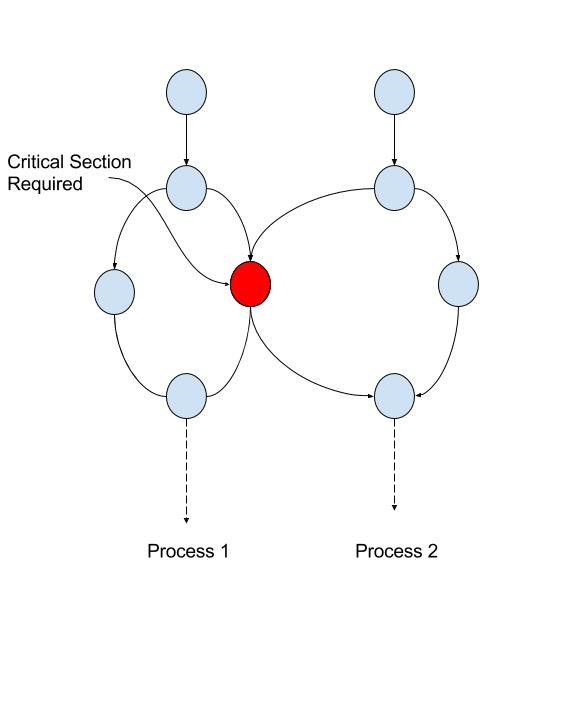
\includegraphics[scale=0.8]{images/critical_section.jpg}
%		Exclusão mútua com espera ociosa:
	\section{Impasses}
		\textit{recurso, introdução a deadlocks, algoritmo do avestruz, detecção e recuperação de deadlocks, evitando deadlocks, prevenção de deadlocks, outras questões}
		
		Em semáforos, o consumidor "acorda" o produtor e vice-versa, para impedir o deadlock.	
		
		Os recursos são executados nessa ordem, solicitar -> usar -> liberar.
		\subsection{Condições para Deadlock}
		\begin{enumerate}
			\item Condição de exclusão mútua
			\item Condição de posse e espera
			\item Condição de não preempção
			\item Condição de espera circular
		\end{enumerate}
		Deadlocks não acontecem em sistemas preemptivos, pois basta salvar o processo e retornar posteriormente.
	\section{Gerenciamento de Memória}'
%z	\section{Entrada e Saída}
\end{document}